%==============================================================
%  EE201 -- Circuit Theory I
%  Lecture 14 : Two-Port Circuits -- slides
%  M. Mert Ankaralı, METU EEE
%
%  Compile:  ./build.sh      (or: pdflatex EE201_Lecture_14_slides.tex, twice)
%  Same colour code as the handout:
%      charge = purple, current = blue, voltage = orange, power = green
%==============================================================
\documentclass[11pt,aspectratio=169]{beamer}

\usepackage{appendixnumberbeamer}
\usepackage[T1]{fontenc}
\usepackage[utf8]{inputenc}
\usepackage[english]{babel}
\usepackage{lmodern}
\usepackage{amsmath,amssymb}
\usepackage{booktabs}
\usepackage{array}
\usepackage{colortbl}
\usepackage{tikz}
\usepackage[american,siunitx]{circuitikz}
\usetikzlibrary{matrix,arrows.meta,positioning,calc,decorations.pathreplacing,decorations.pathmorphing,decorations.markings}
\usetikzlibrary{overlay-beamer-styles}

%-------------------- plain METU-flavoured theme --------------
\usetheme{default}
\usecolortheme{default}
\useinnertheme{rectangles}
\setbeamertemplate{navigation symbols}{}
\setbeamertemplate{itemize items}[square]
\setbeamerfont{frametitle}{size=\large,series=\bfseries}
\setbeamerfont{title}{size=\LARGE,series=\bfseries}

\definecolor{metured}{RGB}{155,27,48}
\definecolor{metugray}{RGB}{88,89,91}
\definecolor{metulight}{RGB}{243,240,241}
\definecolor{ccur}{RGB}{0,102,170}
\definecolor{cvolt}{RGB}{214,120,0}
\definecolor{cpow}{RGB}{23,128,74}
\definecolor{ccharge}{RGB}{124,60,160}
\definecolor{cflux}{RGB}{0,138,138}
\definecolor{copper}{RGB}{184,98,30}

\setbeamercolor{structure}{fg=metured}
\setbeamercolor{frametitle}{fg=metured,bg=}
\setbeamercolor{title}{fg=metured}
\setbeamercolor{normal text}{fg=black!88}
\setbeamercolor{block title}{fg=white,bg=metured}
\setbeamercolor{block body}{bg=metulight}
\setbeamercolor{alerted text}{fg=metured}

\setbeamertemplate{frametitle}{%
  \vspace{0.55em}%
  \usebeamerfont{frametitle}\usebeamercolor[fg]{frametitle}\insertframetitle\par
  \vspace{-0.2em}{\color{metured}\rule{\textwidth}{1pt}}\par\vspace{-0.2em}}

\setbeamertemplate{footline}{%
  \hbox{\begin{beamercolorbox}[wd=\paperwidth,ht=2.4ex,dp=1.4ex,leftskip=1.2em,rightskip=1.2em]{}%
  \tiny\color{metugray}\coursecode\ \textbar\ Lecture 14: Two-Port Circuits
  \hfill \insertframenumber/\inserttotalframenumber
  \end{beamercolorbox}}}

%-------------------- macros ----------------------------------
\newcommand{\coursecode}{EE201}
\newcommand{\term}{Fall 2026--2027}
\newcommand{\Icol}[1]{\textcolor{ccur}{#1}}
\newcommand{\Vcol}[1]{\textcolor{cvolt}{#1}}
\newcommand{\Pcol}[1]{\textcolor{cpow}{#1}}
\newcommand{\Qcol}[1]{\textcolor{ccharge}{#1}}
\newcommand{\Fcol}[1]{\textcolor{cflux}{#1}}
\newcommand{\uni}[1]{\,\mathrm{#1}}
\newcommand{\A}{\uni{A}} \newcommand{\V}{\uni{V}}
\newcommand{\W}{\uni{W}} \newcommand{\J}{\uni{J}}
\newcommand{\Cb}{\uni{C}} \newcommand{\s}{\uni{s}}
\newcommand{\Wb}{\uni{Wb}} \newcommand{\Hy}{\uni{H}}
\newcommand{\Sie}{\uni{S}}


%  voltage sources: smaller + and - inside the circle, further apart
\ctikzset{bipoles/vsourceam/inner plus={\tiny$+$},
          bipoles/vsourceam/inner minus={\tiny$\vphantom{+}-$},
          bipoles/vsourceam/margin=0.85,
          bipoles/cvsourceam/inner plus={\tiny$+$},
          bipoles/cvsourceam/inner minus={\tiny$\vphantom{+}-$},
          bipoles/cvsourceam/margin=0.85}
\ctikzset{bipoles/length=0.9cm, label/align=straight,
          bipoles/generic/height=0.28, bipoles/generic/width=0.62}
\tikzset{
  iar/.style={-{Stealth[length=2.2mm]}, ccur, thick},
  glab/.style={font=\footnotesize, text=metured},
  ttl/.style={font=\scriptsize\bfseries, text=metugray},
  capn/.style={font=\scriptsize, text=metugray, align=center},
  pol/.style={font=\small, text=cvolt},
  nlab/.style={circle, draw=metured, text=metured, font=\scriptsize, inner sep=0.7pt},
  blab/.style={font=\footnotesize, text=black!80},
  gbr/.style={black!75, thick, postaction={decorate, decoration={markings,
      mark=at position 0.56 with {\arrow{Stealth[length=2.5mm]}}}}},
  hal/.style={draw=cpow!60, line width=6pt, opacity=0.35, line cap=round, line join=round},
  halo/.style={circle, fill=metured!16, minimum size=0.95cm},
  elem/.style={draw=metugray, thick, fill=metulight},
  bigarr/.style={-{Stealth[length=3mm]}, very thick, metugray},
}

%-------------------- Lecture 14 circuit macros ---------------
\newcommand{\ohm}{\,\Omega}
\newcommand{\yes}{\textcolor{cpow}{\checkmark}}
\newcommand{\e}[1]{\textcolor{cvolt}{e_{#1}}}
\newcommand{\nd}[1]{\tikz[baseline=(c.base)]\node[nlab](c){#1};}
\newcommand{\gnd}[2]{\draw (#1,#2) -- ++(0,-0.2) node[ground] {};}
\newcommand{\Rin}{R_{\mathrm{in}}}
%  Port variables in colour
\newcommand{\vone}{\Vcol{v_1}}  \newcommand{\vtwo}{\Vcol{v_2}}
\newcommand{\ione}{\Icol{i_1}}  \newcommand{\itwo}{\Icol{i_2}}
\newcommand{\Rm}{\mathbf{R}}  \newcommand{\Gm}{\mathbf{G}}
\newcommand{\Hm}{\mathbf{H}}  \newcommand{\Tm}{\mathbf{T}}
%  Labels beside a vertical element at (#1,#2), a fixed distance to the right (\lR) or left (\lL)
\newcommand{\lR}[3]{\node[anchor=west, xshift=7pt, font=\small] at (#1,#2) {#3};}
\newcommand{\lL}[3]{\node[anchor=east, xshift=-7pt, font=\small] at (#1,#2) {#3};}
\tikzset{tlab/.style={font=\small\bfseries, text=black!80},
         dotm/.style={circle, fill=black, inner sep=0pt, minimum size=4.2pt},
         core/.style={line width=1.1pt, metugray}}

%  Port 1 at terminals x = #1 (top y = #2, bottom y = 0): i_1 into the top terminal, + v_1 -
\newcommand{\pone}[2]{%
  \draw (#1,#2) node[ocirc] {}; \draw (#1,0) node[ocirc] {};
  \draw[iar] (#1+0.2,#2+0.28) -- (#1+0.75,#2+0.28); \node[font=\small, text=ccur] at (#1+0.48,#2+0.58) {$i_1$};
  \node[pol] at (#1+0.3,0.72*#2) {$+$}; \node[pol] at (#1+0.3,0.22*#2) {$-$};
  \node[font=\small, text=cvolt] at (#1+0.32,0.47*#2) {$v_1$};}
%  Port 2 at terminals x = #1: i_2 into the top terminal (pointing left), + v_2 -
\newcommand{\ptwo}[2]{%
  \draw (#1,#2) node[ocirc] {}; \draw (#1,0) node[ocirc] {};
  \draw[iar] (#1-0.2,#2+0.28) -- (#1-0.75,#2+0.28); \node[font=\small, text=ccur] at (#1-0.48,#2+0.58) {$i_2$};
  \node[pol] at (#1-0.3,0.72*#2) {$+$}; \node[pol] at (#1-0.3,0.22*#2) {$-$};
  \node[font=\small, text=cvolt] at (#1-0.32,0.47*#2) {$v_2$};}
%  A two-port box (text #1) with both ports
\newcommand{\tpbox}[1]{%
  \draw[elem] (1.0,-0.2) rectangle (3.4,2.2);
  \node[align=center, font=\small] at (2.2,1.0) {#1};
  \draw (0,1.8) -- (1.0,1.8); \draw (0,0) -- (1.0,0);
  \draw (3.4,1.8) -- (4.4,1.8); \draw (3.4,0) -- (4.4,0);
  \pone{0}{1.8} \ptwo{4.4}{1.8}}
%  A one-port box with a resistor-like port (for the review)
\newcommand{\opbox}[1]{%
  \draw[elem] (0,0) rectangle (1.9,2);
  \node[align=center, font=\small] at (0.95,1) {#1};
  \draw (1.9,1.7) -- (3.0,1.7) node[ocirc] {}; \draw (1.9,0.3) -- (3.0,0.3) node[ocirc] {};
  \draw[iar] (2.75,1.95) -- (2.2,1.95); \node[font=\small, text=ccur] at (2.48,2.25) {$i$};
  \node[pol] at (2.6,1.4) {$+$}; \node[pol] at (2.6,0.6) {$-$};
  \node[font=\small, text=cvolt] at (2.6,1.0) {$v$};}

%  Example 14.1: R_1 across port 1, R_2 across port 2 (no coupling)
\newcommand{\exTriv}{%
  \draw (0,1.8) -- (1.5,1.8); \draw (0,0) -- (1.5,0);
  \draw (1.5,1.8) to[R] (1.5,0); \lR{1.5}{0.9}{$R_1$}
  \draw (4.1,1.8) to[R] (4.1,0); \lL{4.1}{0.9}{$R_2$}
  \draw (4.1,1.8) -- (5.6,1.8); \draw (4.1,0) -- (5.6,0);
  \draw[dashed, metugray] (1.0,-0.45) rectangle (4.6,2.45);
  \pone{0}{1.8} \ptwo{5.6}{1.8}}

%  Example 14.2: R_1 (series), R_2 (shunt), CCVS 2 i_1 (+ on the left).
%  #1 = 0: both ports;  1: i_2 = 0 (port 2 open);  2: i_1 = 0 (port 1 open);  3: v_2 = 0 (port 2 shorted)
%  #2, #3: labels of R_1, R_2
\newcommand{\exTee}[4][2]{%
  \draw (0,2.2) -- (0.9,2.2) to[R, l=#3] (2.6,2.2) -- (4.3,2.2);
  \draw (4.3,2.2) to[american controlled voltage source, l=$\Vcol{#1\,i_1}$] (5.9,2.2) -- (6.9,2.2);
  \draw (2.6,2.2) to[R] (2.6,0); \lR{2.6}{1.1}{#4}
  \draw (0,0) -- (6.9,0);
  \fill (2.6,2.2) circle (1.7pt); \fill (2.6,0) circle (1.7pt);
  \ifcase#2
    \pone{0}{2.2} \ptwo{6.9}{2.2}
  \or
    \pone{0}{2.2}
    \draw (6.9,2.2) node[ocirc] {}; \draw (6.9,0) node[ocirc] {};
    \node[pol] at (6.6,1.6) {$+$}; \node[pol] at (6.6,0.5) {$-$};
    \node[font=\small, text=cvolt] at (6.58,1.05) {$v_2$};
    \node[font=\small, text=ccur, anchor=west] at (7.05,2.2) {$i_2 = 0$};
  \or
    \draw (0,2.2) node[ocirc] {}; \draw (0,0) node[ocirc] {};
    \node[pol] at (0.3,1.6) {$+$}; \node[pol] at (0.3,0.5) {$-$};
    \node[font=\small, text=cvolt] at (0.32,1.05) {$v_1$};
    \node[font=\small, text=ccur, anchor=east] at (-0.15,2.2) {$i_1 = 0$};
    \ptwo{6.9}{2.2}
  \or
    \pone{0}{2.2}
    \draw (6.9,2.2) -- (6.9,0);
    \draw[iar] (6.65,2.5) -- (6.1,2.5); \node[font=\small, text=ccur] at (6.38,2.8) {$i_2$};
    \node[font=\small, text=cvolt, anchor=west] at (7.05,1.1) {$v_2 = 0$};
  \fi}

%  Ideal transformer N_1 : N_2 as a two-port (coils at x = 1.4 and 3.0, height 1.8)
\newcommand{\xfmr}[2]{%
  \begin{scope}[xshift=#1 cm]
    \ctikzset{bipoles/length=1.2cm}
    \draw (0,0) to[L] (0,#2);
    \draw (1.6,#2) to[L] (1.6,0);
    \draw[core] (0.72,-0.05) -- (0.72,#2+0.05);
    \draw[core] (0.88,-0.05) -- (0.88,#2+0.05);
    \node[dotm] at (0.36,#2-0.2) {};
    \node[dotm] at (1.24,#2-0.2) {};
  \end{scope}}
\newcommand{\exXf}{%
  \draw (0,1.8) -- (1.4,1.8); \draw (0,0) -- (1.4,0);
  \xfmr{1.4}{1.8}
  \draw (3.0,1.8) -- (4.4,1.8); \draw (3.0,0) -- (4.4,0);
  \node[font=\small] at (2.2,2.2) {$N_1 : N_2$};
  \pone{0}{1.8} \ptwo{4.4}{1.8}}
\newcommand{\Rth}{R_{\mathrm{th}}}

%  Meters drawn upright: vertical (x, ytop, ybot, letter, label right) and horizontal (xl, xr, y, letter, label above)
\newcommand{\vmeter}[5]{%
  \draw (#1,#2) -- (#1,{(#2+#3)/2+0.32}); \draw (#1,{(#2+#3)/2-0.32}) -- (#1,#3);
  \node[circle, draw, thick, minimum size=0.64cm, inner sep=0pt, font=\small\bfseries] at (#1,{(#2+#3)/2}) {#4};
  \node[anchor=west, font=\small] at ({#1+0.38},{(#2+#3)/2}) {#5};}
\newcommand{\hmeter}[5]{%
  \draw (#1,#3) -- ({(#1+#2)/2-0.32},#3); \draw ({(#1+#2)/2+0.32},#3) -- (#2,#3);
  \node[circle, draw, thick, minimum size=0.64cm, inner sep=0pt, font=\small\bfseries] at ({(#1+#2)/2},#3) {#4};
  \node[anchor=south, font=\small] at ({(#1+#2)/2},{#3+0.36}) {#5};}
%  Test bench for a two-port in a box. #1 = 0: open-circuit test (current source at port 1,
%  voltmeters at both ports); 1: short-circuit test (voltage source at port 1, ammeters)
\newcommand{\bench}[1]{%
  \draw[thick, fill=gray!8] (3.0,-0.2) rectangle (5.0,2.4);
  \node[font=\large] at (4.0,1.1) {$N$};
  \draw (3.0,2.0) -- (2.6,2.0); \draw (3.0,0.2) -- (2.6,0.2);
  \draw (5.0,2.0) -- (5.4,2.0); \draw (5.0,0.2) -- (5.4,0.2);
  \foreach \p in {(2.6,2.0),(2.6,0.2),(5.4,2.0),(5.4,0.2)} \draw \p node[ocirc] {};
  \ifcase#1
    \draw (0,0.2) to[american current source, l=$\Icol{i_1}$] (0,2.0) -- (2.6,2.0);
    \draw (0,0.2) -- (2.6,0.2);
    \vmeter{1.5}{2.0}{0.2}{V}{$\Vcol{v_1}$}
    \fill (1.5,2.0) circle (1.6pt); \fill (1.5,0.2) circle (1.6pt);
    \draw (5.4,2.0) -- (6.6,2.0); \draw (5.4,0.2) -- (6.6,0.2);
    \vmeter{6.6}{2.0}{0.2}{V}{$\Vcol{v_2}$}
    \node[font=\small, text=ccur, anchor=south] at (6.0,2.05) {$i_2 = 0$};
  \or
    \draw (0,2.0) to[american voltage source, l_=$\Vcol{v_1}$] (0,0.2);
    \hmeter{0}{2.6}{2.0}{A}{$\Icol{i_1}$}
    \draw (0,0.2) -- (2.6,0.2);
    \draw (5.4,2.0) -- (6.6,2.0); \draw (5.4,0.2) -- (6.6,0.2);
    \vmeter{6.6}{2.0}{0.2}{A}{$\Icol{i_2}$}
    \node[font=\small, text=cvolt, anchor=south] at (6.0,2.05) {$v_2 = 0$};
  \fi}
\title{Lecture 14: Two-Port Circuits}
\subtitle{EE201 -- Circuit Theory I}
\author{M. Mert Ankaral{\i}}
\institute{\small Department of Electrical and Electronics Engineering\\
           Middle East Technical University}
\date{}

%  Roadmap icons (1-5): a two-port box with the letter of its matrix
\newcommand{\rmicon}[1]{%
  \draw[thick] (-0.8,-0.7) rectangle (0.8,0.7);
  \draw (-1.6,0.5) node[ocirc] {} -- (-0.8,0.5); \draw (-1.6,-0.5) node[ocirc] {} -- (-0.8,-0.5);
  \draw (0.8,0.5) -- (1.6,0.5) node[ocirc] {}; \draw (0.8,-0.5) -- (1.6,-0.5) node[ocirc] {};
  \node[font=\LARGE\bfseries] at (0,0) {\ifcase#1\or$\mathbf{R}$\or$\mathbf{G}$\or$\mathbf{H}$\or$\mathbf{T}$\or$P$\fi};}
%  Stops 1-7: station of stop k = \rmst{k}
\newcommand{\rmst}[1]{\ifcase#1\or1\or1\or2\or3\or3\or4\or5\fi}
\newcommand{\rmstation}[4]{%
  \ifnum#1<\rmS\relax
    \node[circle, fill=cpow, text=white, inner sep=0pt, minimum size=5.4mm, font=\scriptsize\bfseries] at (#2,0) {\checkmark};
    \node[text=black!40, font=\small\bfseries, align=center, anchor=south, inner sep=1pt] at (#2,0.36) {#3};
  \else\ifnum#1=\rmS\relax
    \node[circle, fill=metured, text=white, inner sep=0pt, minimum size=6.2mm, font=\small\bfseries] at (#2,0) {#1};
    \node[text=metured, font=\small\bfseries, align=center, anchor=south, inner sep=1pt] at (#2,0.36) {#3};
  \else
    \node[circle, draw=metugray, fill=white, text=metugray, inner sep=0pt, minimum size=5.4mm, font=\scriptsize\bfseries] at (#2,0) {#1};
    \node[font=\small\bfseries, align=center, anchor=south, inner sep=1pt] at (#2,0.36) {#3};
  \fi\fi
  \begin{scope}[shift={(#2,1.75)}, scale=0.42, transform shape]
    \ifnum#1>\rmS\relax\begin{scope}[opacity=0.5]\rmicon{#4}\end{scope}\else\rmicon{#4}\fi
  \end{scope}}
%  #1 first stop, #2 last stop covered by this item, #3 x, #4 y, #5 text
\newcommand{\rmsub}[5]{%
  \ifnum#2<\rmcur\relax
    \node[text width=2.5cm, align=center, font=\footnotesize, text=black!40] at (#3,#4) {#5\ \textcolor{cpow}{\checkmark}};
  \else\ifnum#1>\rmcur\relax
    \node[text width=2.5cm, align=center, font=\footnotesize] at (#3,#4) {#5};
  \else
    \node[text width=2.5cm, align=center, font=\footnotesize\bfseries, text=metured,
          draw=metured, rounded corners=2pt, inner sep=2pt] at (#3,#4) {#5};
  \fi\fi}
\newcommand{\roadmapframe}[1]{%
  \begin{frame}{Roadmap}
    \def\rmcur{#1}\edef\rmS{\rmst{#1}}%
    \vfill
    \centering
    \begin{tikzpicture}
      \draw[metugray!45, line width=3pt, -{Stealth[length=2.6mm, width=3.2mm]}] (0,0) -- (13.5,0);
      \rmstation{1}{1.35}{Resistance\\ matrix}{1}
      \rmstation{2}{4.05}{Conductance\\ matrix}{2}
      \rmstation{3}{6.75}{Hybrid\\ matrices}{3}
      \rmstation{4}{9.45}{Transmission\\ matrix}{4}
      \rmstation{5}{12.15}{Power}{5}
      \rmsub{1}{1}{1.35}{-0.8}{$\mathbf{v} = \mathbf{R}\,\mathbf{i}$}
      \rmsub{2}{2}{1.35}{-1.4}{open-circuit tests}
      \rmsub{3}{3}{4.05}{-0.8}{$\mathbf{i} = \mathbf{G}\,\mathbf{v}$}
      \rmsub{3}{3}{4.05}{-1.4}{short-circuit tests}
      \rmsub{4}{4}{6.75}{-0.8}{$\mathbf{H}$ and $\mathbf{H}'$}
      \rmsub{4}{4}{6.75}{-1.4}{ideal transformer}
      \rmsub{6}{6}{9.45}{-0.8}{$\vtwo$ and $-\itwo$}
      \rmsub{6}{6}{9.45}{-1.4}{ideal transformer}
      \rmsub{7}{7}{12.15}{-0.8}{$\vone\ione + \vtwo\itwo$}
      \rmsub{7}{7}{12.15}{-1.4}{passive, active}
    \end{tikzpicture}
    \vfill
    \mbox{}
    \vfill
  \end{frame}}
\begin{document}

%--------------------------------------------------------------
\begin{frame}[plain]
  \titlepage
  \vspace{-1.2em}
  \begin{center}\scriptsize\color{metugray}
    \Icol{$\blacksquare$}~current \quad \Vcol{$\blacksquare$}~voltage, node voltage $e$
  \end{center}
\end{frame}

%--------------------------------------------------------------
\begin{frame}{Review: one-ports}
  \vfill
  \begin{columns}[c,onlytextwidth]
    \begin{column}{0.42\textwidth}
      \centering
      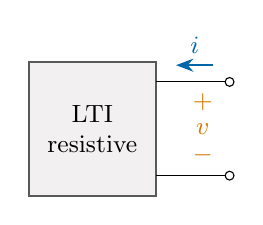
\begin{tikzpicture}[scale=0.85]
        \opbox{LTI\\resistive}
      \end{tikzpicture}
    \end{column}
    \begin{column}{0.56\textwidth}
      \begin{itemize}\itemsep8pt
        \item No independent sources: \ $\Vcol{v} = \Rin\,\Icol{i}$
        \item With independent sources: \ $\Vcol{v} = \Rth\,\Icol{i} + \Vcol{v_{\mathrm{th}}}$
      \end{itemize}
    \end{column}
  \end{columns}
  \vfill
\end{frame}

%==============================================================
\roadmapframe{1}

%--------------------------------------------------------------
\begin{frame}{Motivation: two ports}
  \vfill
  \begin{center}
    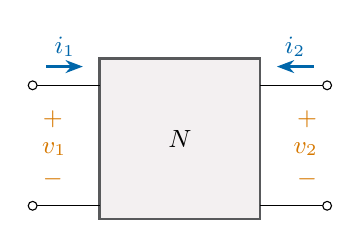
\begin{tikzpicture}[scale=0.85]
      \tpbox{$N$}
    \end{tikzpicture}
  \end{center}
  \vfill
  \begin{itemize}\itemsep8pt
    \item $N$: LTI resistive, no independent sources
    \item An input and an output: an amplifier, a transformer, a filter
    \item One-port: $\Vcol{v} = R\,\Icol{i}$ with scalars
    \item<2-> Two-port: $\mathbf{v} = \mathbf{R}\,\mathbf{i}$ with vectors in $\mathbb{R}^2$ and a $2 \times 2$ matrix
  \end{itemize}
  \vfill
\end{frame}

%--------------------------------------------------------------
\begin{frame}{The port variables}
  \begin{columns}[c,onlytextwidth]
    \begin{column}{0.5\textwidth}
      \centering
      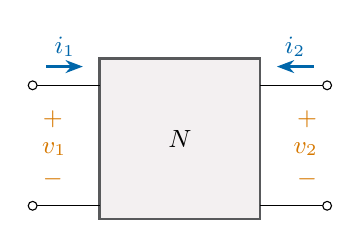
\begin{tikzpicture}[scale=0.85]
        \tpbox{$N$}
      \end{tikzpicture}
    \end{column}
    \begin{column}{0.48\textwidth}
      \begin{itemize}\itemsep8pt
        \item Each port: the current enters at $+$ and leaves at $-$
        \item Four variables: $\vone$, $\ione$, $\vtwo$, $\itwo$
        \item<2-> Two equations: two variables in terms of the other two
      \end{itemize}
    \end{column}
  \end{columns}
  \vfill
  \onslide<3->{%
  \begin{center}
    \renewcommand{\arraystretch}{1.3}
    \begin{tabular}{@{}lll@{}}
      \toprule
      given & find & matrix\\
      \midrule
      $\ione$, $\itwo$ & $\vone$, $\vtwo$ & resistance $\Rm$\\
      $\vone$, $\vtwo$ & $\ione$, $\itwo$ & conductance $\Gm$\\
      $\ione$, $\vtwo$ & $\vone$, $\itwo$ & hybrid $\Hm$\\
      $\vtwo$, $-\itwo$ & $\vone$, $\ione$ & transmission $\Tm$\\
      \bottomrule
    \end{tabular}
  \end{center}}
\end{frame}

%--------------------------------------------------------------
\begin{frame}{The resistance matrix}
  \vfill
  \begin{columns}[c,onlytextwidth]
    \begin{column}{0.46\textwidth}
      \centering
      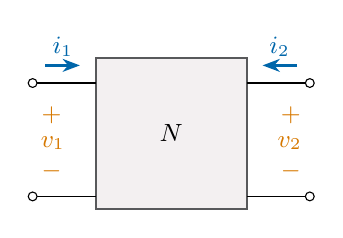
\begin{tikzpicture}[scale=0.8]
        \tpbox{$N$}
      \end{tikzpicture}
    \end{column}
    \begin{column}{0.52\textwidth}
      $\vone = r_{11}\,\ione + r_{12}\,\itwo$\\[6pt]
      $\vtwo = r_{21}\,\ione + r_{22}\,\itwo$\\[14pt]
      \onslide<2->{%
      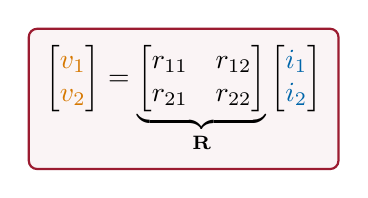
\begin{tikzpicture}
        \node[draw=metured, thick, fill=metured!5, rounded corners=3pt, inner sep=6pt]
          {$\begin{bmatrix} \vone\\ \vtwo \end{bmatrix}
            = \underbrace{\begin{bmatrix} r_{11} & r_{12}\\ r_{21} & r_{22} \end{bmatrix}}_{\Rm}
              \begin{bmatrix} \ione\\ \itwo \end{bmatrix}$};
      \end{tikzpicture}}
    \end{column}
  \end{columns}
  \vfill
\end{frame}

%--------------------------------------------------------------
\begin{frame}{Example 14.1: two separate resistors}
  \begin{columns}[c,onlytextwidth]
    \begin{column}{0.52\textwidth}
      \centering
      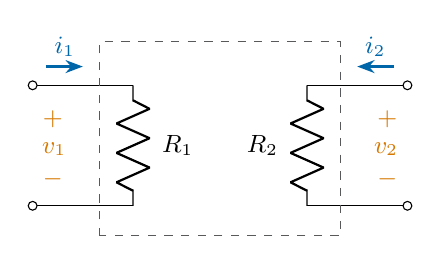
\begin{tikzpicture}[scale=0.85]
        \exTriv
      \end{tikzpicture}
    \end{column}
    \begin{column}{0.46\textwidth}
      $\Rm = \ ?$\\[14pt]
      \onslide<2->{%
      $\vone = R_1\,\ione + 0\cdot\itwo$\\[4pt]
      $\vtwo = 0\cdot\ione + R_2\,\itwo$\\[12pt]
      $\Rm = \begin{bmatrix} R_1 & 0\\ 0 & R_2 \end{bmatrix}$\\[10pt]
      No coupling: \ $r_{12} = r_{21} = 0$}
    \end{column}
  \end{columns}
\end{frame}

%--------------------------------------------------------------
\begin{frame}{Example 14.2: a dependent source inside}
  \vfill
  \begin{center}
    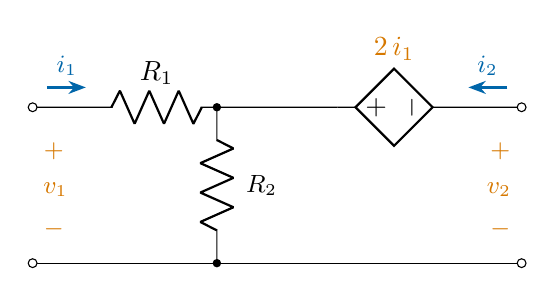
\begin{tikzpicture}[scale=0.9]
      \exTee{0}{$R_1$}{$R_2$}
    \end{tikzpicture}
  \end{center}
  \vfill
  \begin{center}
    $\Rm = \ ?$
  \end{center}
  \vfill
\end{frame}

%--------------------------------------------------------------
\begin{frame}{Example 14.2: KVL}
  \begin{columns}[c,onlytextwidth]
    \begin{column}{0.5\textwidth}
      \centering
      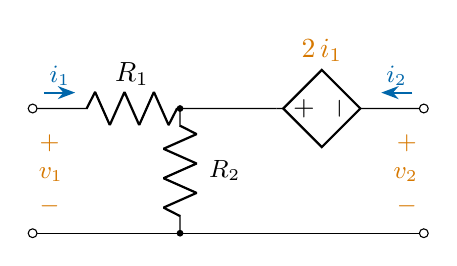
\begin{tikzpicture}[scale=0.72]
        \exTee{0}{$R_1$}{$R_2$}
      \end{tikzpicture}
    \end{column}
    \begin{column}{0.48\textwidth}
      $R_2$ carries $\ione + \itwo$\\[8pt]
      $\vone = R_1\,\ione + R_2(\ione + \itwo)$\\[6pt]
      $\vtwo = -2\,\ione + R_2(\ione + \itwo)$\\[14pt]
      \onslide<2->{%
      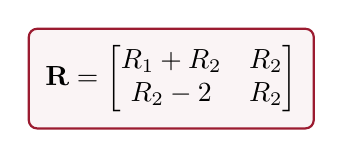
\begin{tikzpicture}
        \node[draw=metured, thick, fill=metured!5, rounded corners=3pt, inner sep=6pt]
          {$\Rm = \begin{bmatrix} R_1 + R_2 & R_2\\ R_2 - 2 & R_2 \end{bmatrix}$};
      \end{tikzpicture}\\[8pt]
      {\small $r_{12} \neq r_{21}$: the dependent source}}
    \end{column}
  \end{columns}
\end{frame}

%==============================================================
\roadmapframe{2}

%--------------------------------------------------------------
\begin{frame}{The entries from two tests}
  \vfill
  \begin{center}
    \textbf{Port 2 open:} \ $\itwo = 0$\\[8pt]
    $\begin{bmatrix} \vone\\ \vtwo \end{bmatrix}
     = \begin{bmatrix} \alert{r_{11}} & r_{12}\\ \alert{r_{21}} & r_{22} \end{bmatrix}
       \begin{bmatrix} \ione\\ 0 \end{bmatrix}
     = \begin{bmatrix} r_{11}\,\ione\\ r_{21}\,\ione \end{bmatrix}$
    \quad $\Rightarrow$ \quad
    $\displaystyle r_{11} = \frac{\vone}{\ione}, \quad r_{21} = \frac{\vtwo}{\ione}$\\[4pt]
    {\small the first column: \ $r_{11}$ input resistance, \ $r_{21}$ transfer resistance}
  \end{center}
  \vfill
  \onslide<2->{%
  \begin{center}
    \textbf{Port 1 open:} \ $\ione = 0$\\[8pt]
    $\begin{bmatrix} \vone\\ \vtwo \end{bmatrix}
     = \begin{bmatrix} r_{11} & \alert{r_{12}}\\ r_{21} & \alert{r_{22}} \end{bmatrix}
       \begin{bmatrix} 0\\ \itwo \end{bmatrix}
     = \begin{bmatrix} r_{12}\,\itwo\\ r_{22}\,\itwo \end{bmatrix}$
    \quad $\Rightarrow$ \quad
    $\displaystyle r_{12} = \frac{\vone}{\itwo}, \quad r_{22} = \frac{\vtwo}{\itwo}$\\[4pt]
    {\small the second column: \ $r_{12}$ transfer resistance, \ $r_{22}$ input resistance}
  \end{center}}
  \vfill
\end{frame}

%--------------------------------------------------------------
\begin{frame}{Example 14.2 revisited: port 2 open}
  \begin{columns}[c,onlytextwidth]
    \begin{column}{0.52\textwidth}
      \centering
      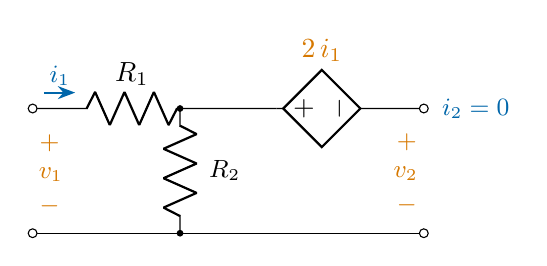
\begin{tikzpicture}[scale=0.72]
        \exTee{1}{$R_1$}{$R_2$}
      \end{tikzpicture}
    \end{column}
    \begin{column}{0.46\textwidth}
      No current through the dependent source\\[8pt]
      $\vone = (R_1 + R_2)\,\ione$ \ $\Rightarrow$ \ $r_{11} = R_1 + R_2$\\[6pt]
      $\vtwo = -2\,\ione + R_2\,\ione$ \ $\Rightarrow$ \ $r_{21} = R_2 - 2$
    \end{column}
  \end{columns}
\end{frame}

%--------------------------------------------------------------
\begin{frame}{Example 14.2 revisited: port 1 open}
  \begin{columns}[c,onlytextwidth]
    \begin{column}{0.52\textwidth}
      \centering
      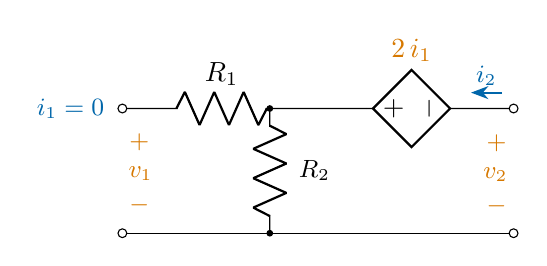
\begin{tikzpicture}[scale=0.72]
        \exTee{2}{$R_1$}{$R_2$}
      \end{tikzpicture}
    \end{column}
    \begin{column}{0.46\textwidth}
      No current in $R_1$; the dependent source is $0$\\[8pt]
      $\vone = R_2\,\itwo$ \ $\Rightarrow$ \ $r_{12} = R_2$\\[6pt]
      $\vtwo = R_2\,\itwo$ \ $\Rightarrow$ \ $r_{22} = R_2$\\[12pt]
      \onslide<2->{The same $\Rm$ \ \yes}
    \end{column}
  \end{columns}
\end{frame}

%==============================================================
\roadmapframe{3}

%--------------------------------------------------------------
\begin{frame}{The conductance matrix}
  \vfill
  \begin{center}
    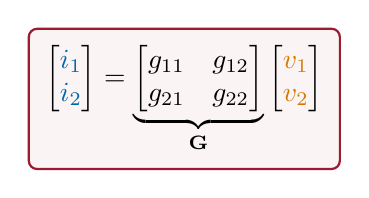
\begin{tikzpicture}
      \node[draw=metured, thick, fill=metured!5, rounded corners=3pt, inner sep=6pt]
        {$\begin{bmatrix} \ione\\ \itwo \end{bmatrix}
          = \underbrace{\begin{bmatrix} g_{11} & g_{12}\\ g_{21} & g_{22} \end{bmatrix}}_{\Gm}
            \begin{bmatrix} \vone\\ \vtwo \end{bmatrix}$};
    \end{tikzpicture}\\[16pt]
    \onslide<2->{When $\Rm^{-1}$ exists: \ $\Gm = \Rm^{-1}$}
  \end{center}
  \vfill
\end{frame}

%--------------------------------------------------------------
\begin{frame}{The entries from two short-circuit tests}
  \vfill
  \begin{center}
    \textbf{Port 2 shorted:} \ $\vtwo = 0$\\[8pt]
    $\begin{bmatrix} \ione\\ \itwo \end{bmatrix}
     = \begin{bmatrix} \alert{g_{11}} & g_{12}\\ \alert{g_{21}} & g_{22} \end{bmatrix}
       \begin{bmatrix} \vone\\ 0 \end{bmatrix}
     = \begin{bmatrix} g_{11}\,\vone\\ g_{21}\,\vone \end{bmatrix}$
    \quad $\Rightarrow$ \quad
    $\displaystyle g_{11} = \frac{\ione}{\vone}, \quad g_{21} = \frac{\itwo}{\vone}$\\[4pt]
    {\small the first column: \ $g_{11}$ input conductance, \ $g_{21}$ transfer conductance}
  \end{center}
  \vfill
  \onslide<2->{%
  \begin{center}
    \textbf{Port 1 shorted:} \ $\vone = 0$\\[8pt]
    $\begin{bmatrix} \ione\\ \itwo \end{bmatrix}
     = \begin{bmatrix} g_{11} & \alert{g_{12}}\\ g_{21} & \alert{g_{22}} \end{bmatrix}
       \begin{bmatrix} 0\\ \vtwo \end{bmatrix}
     = \begin{bmatrix} g_{12}\,\vtwo\\ g_{22}\,\vtwo \end{bmatrix}$
    \quad $\Rightarrow$ \quad
    $\displaystyle g_{12} = \frac{\ione}{\vtwo}, \quad g_{22} = \frac{\itwo}{\vtwo}$\\[4pt]
    {\small the second column: \ $g_{12}$ transfer conductance, \ $g_{22}$ input conductance}
  \end{center}}
  \vfill
\end{frame}

%--------------------------------------------------------------
\begin{frame}{Example 14.3: $\Gm$ for Example 14.2}
  \begin{columns}[c,onlytextwidth]
    \begin{column}{0.5\textwidth}
      \centering
      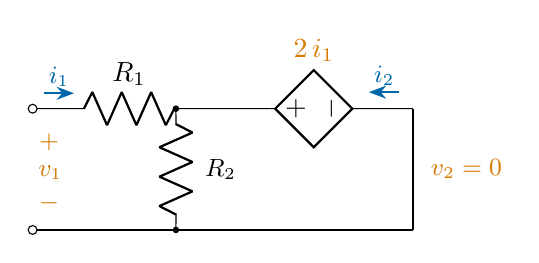
\begin{tikzpicture}[scale=0.7]
        \exTee{3}{$R_1$}{$R_2$}
      \end{tikzpicture}\\[6pt]
      {\small Port 2 shorted: \ $\vtwo = 0$}
    \end{column}
    \begin{column}{0.48\textwidth}
      \textbf{Mesh 1:} \ $-\vone + R_1\,\ione + R_2(\ione + \itwo) = 0$\\[6pt]
      \textbf{Mesh 2:} \ $-2\,\ione + R_2(\ione + \itwo) = 0$\\[12pt]
      \onslide<2->{%
      $\begin{bmatrix} R_1 + R_2 & R_2\\ R_2 - 2 & R_2 \end{bmatrix}
       \begin{bmatrix} \ione\\ \itwo \end{bmatrix}
       = \begin{bmatrix} 1\\ 0 \end{bmatrix} \vone$\\[8pt]
      The matrix is $\Rm$}
    \end{column}
  \end{columns}
\end{frame}

%--------------------------------------------------------------
\begin{frame}{Example 14.3: the result}
  \vfill
  \begin{center}
    $\Delta = \det \Rm = (R_1 + R_2)\,R_2 - R_2(R_2 - 2) = R_2\,(R_1 + 2)$\\[14pt]
    $\displaystyle g_{11} = \frac{R_2}{\Delta} = \frac{1}{R_1 + 2}, \qquad g_{21} = \frac{2 - R_2}{\Delta}$\\[14pt]
    \onslide<2->{%
    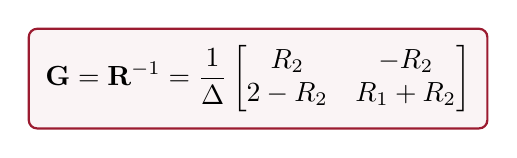
\begin{tikzpicture}
      \node[draw=metured, thick, fill=metured!5, rounded corners=3pt, inner sep=6pt]
        {$\displaystyle \Gm = \Rm^{-1} = \frac{1}{\Delta}
          \begin{bmatrix} R_2 & -R_2\\ 2 - R_2 & R_1 + R_2 \end{bmatrix}$};
    \end{tikzpicture}}
  \end{center}
  \vfill
  \onslide<3->{%
  \begin{center}
    \small $\Rm$ or $\Gm$ need not exist
  \end{center}}
  \vfill
\end{frame}

%==============================================================
\roadmapframe{4}

%--------------------------------------------------------------
\begin{frame}{Hybrid matrices}
  \vfill
  \begin{center}
    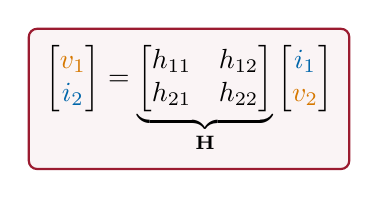
\begin{tikzpicture}
      \node[draw=metured, thick, fill=metured!5, rounded corners=3pt, inner sep=6pt]
        {$\begin{bmatrix} \vone\\ \itwo \end{bmatrix}
          = \underbrace{\begin{bmatrix} h_{11} & h_{12}\\ h_{21} & h_{22} \end{bmatrix}}_{\Hm}
            \begin{bmatrix} \ione\\ \vtwo \end{bmatrix}$};
    \end{tikzpicture}
    \qquad
    \onslide<2->{%
    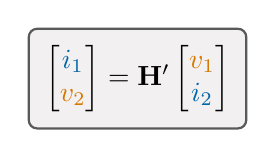
\begin{tikzpicture}
      \node[draw=metugray, thick, fill=metulight, rounded corners=3pt, inner sep=6pt]
        {$\begin{bmatrix} \ione\\ \vtwo \end{bmatrix}
          = \Hm' \begin{bmatrix} \vone\\ \itwo \end{bmatrix}$};
    \end{tikzpicture}}
  \end{center}
  \vfill
  \begin{itemize}\itemsep8pt
    \item<2-> $\Hm' = \Hm^{-1}$ \ when the inverse exists
    \item<3-> $h_{11}$, $h_{21}$: \ port 2 shorted, $\vtwo = 0$
    \item<3-> $h_{12}$, $h_{22}$: \ port 1 open, $\ione = 0$
  \end{itemize}
  \vfill
\end{frame}

%--------------------------------------------------------------
\begin{frame}{Example 14.4: $\Hm$ of a circuit}
  \vfill
  \begin{center}
    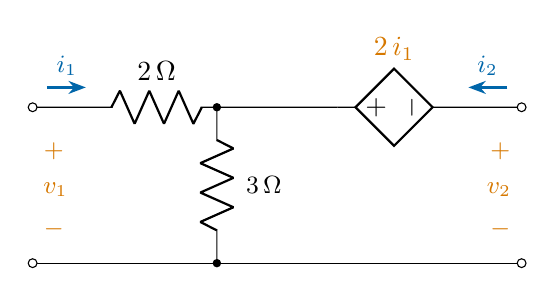
\begin{tikzpicture}[scale=0.9]
      \exTee{0}{$2\ohm$}{$3\ohm$}
    \end{tikzpicture}
  \end{center}
  \vfill
  \begin{center}
    The circuit of Example 14.2 with numbers: \ $\Hm = \ ?$
  \end{center}
  \vfill
\end{frame}

%--------------------------------------------------------------
\begin{frame}{Example 14.4: two tests}
  \begin{columns}[t,onlytextwidth]
    \begin{column}{0.48\textwidth}
      \centering
      \textbf{Port 2 shorted:} \ $\vtwo = 0$\\[6pt]
      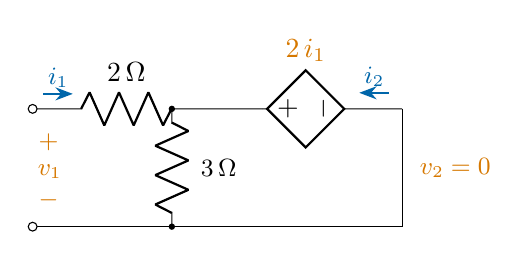
\begin{tikzpicture}[scale=0.68]
        \exTee{3}{$2\ohm$}{$3\ohm$}
      \end{tikzpicture}\\[4pt]
      \raggedright
      Mesh 2: \ $-2\,\ione + 3(\ione + \itwo) = 0$\\[2pt]
      \hspace*{1em}$\Rightarrow$ \ $\itwo = -\tfrac13\,\ione$\\[4pt]
      Mesh 1: \ $\vone = 2\,\ione + 3(\ione + \itwo) = 4\,\ione$\\[6pt]
      $h_{11} = 4\ohm$, \quad $h_{21} = -\tfrac13$
    \end{column}
    \begin{column}{0.48\textwidth}
      \centering
      \onslide<2->{%
      \textbf{Port 1 open:} \ $\ione = 0$\\[6pt]
      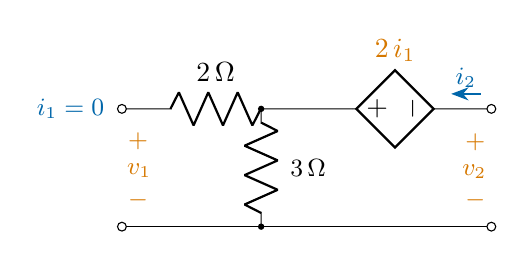
\begin{tikzpicture}[scale=0.68]
        \exTee{2}{$2\ohm$}{$3\ohm$}
      \end{tikzpicture}\\[4pt]
      \raggedright
      The dependent source is $0$: \ $\vtwo = 3\,\itwo$\\[2pt]
      \hspace*{1em}$\Rightarrow$ \ $\itwo = \tfrac13\,\vtwo$\\[4pt]
      $\vone = 3\,\itwo = \vtwo$\\[6pt]
      $h_{12} = 1$, \quad $h_{22} = \tfrac13\,\mathrm{S}$}
    \end{column}
  \end{columns}
\end{frame}

%--------------------------------------------------------------
\begin{frame}{Example 14.4: the result}
  \vfill
  \begin{center}
    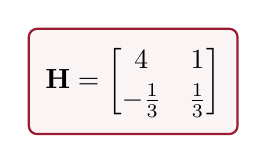
\begin{tikzpicture}
      \node[draw=metured, thick, fill=metured!5, rounded corners=3pt, inner sep=6pt]
        {$\Hm = \begin{bmatrix} 4 & 1\\[2pt] -\tfrac13 & \tfrac13 \end{bmatrix}$};
    \end{tikzpicture}
  \end{center}
  \vfill
  \begin{itemize}\itemsep8pt
    \item Units: $h_{11}$ in $\Omega$, $h_{22}$ in S, $h_{12}$ and $h_{21}$ without units
    \item Check with $\Rm = \begin{bmatrix} 5 & 3\\ 1 & 3 \end{bmatrix}$ from Example 14.2 \ \yes
  \end{itemize}
  \vfill
\end{frame}

%--------------------------------------------------------------
\begin{frame}{Example 14.5: the ideal transformer}
  \begin{columns}[c,onlytextwidth]
    \begin{column}{0.48\textwidth}
      \centering
      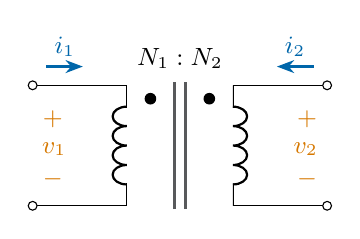
\begin{tikzpicture}[scale=0.85]
        \exXf
      \end{tikzpicture}\\[8pt]
      $\dfrac{\vone}{N_1} = \dfrac{\vtwo}{N_2}$, \quad $N_1\,\ione + N_2\,\itwo = 0$
    \end{column}
    \begin{column}{0.5\textwidth}
      $\Hm = \ ?$ \quad $\Rm = \ ?$\\[12pt]
      \onslide<2->{%
      With $n = N_1/N_2$:\\[4pt]
      $\vone = n\,\vtwo$, \quad $\itwo = -n\,\ione$\\[10pt]
      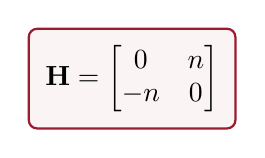
\begin{tikzpicture}
        \node[draw=metured, thick, fill=metured!5, rounded corners=3pt, inner sep=6pt]
          {$\Hm = \begin{bmatrix} 0 & n\\ -n & 0 \end{bmatrix}$};
      \end{tikzpicture}\\[10pt]}
      \onslide<3->{%
      Ports open: $\ione = \itwo = 0$, but $\vone$, $\vtwo$ are free\\[4pt]
      No $\Rm$, no $\Gm$}
    \end{column}
  \end{columns}
\end{frame}

%==============================================================
\roadmapframe{6}

%--------------------------------------------------------------
\begin{frame}{The transmission matrix}
  \vfill
  \begin{center}
    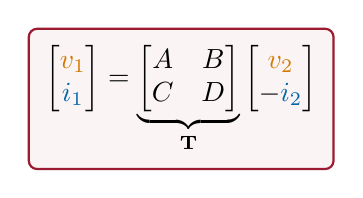
\begin{tikzpicture}
      \node[draw=metured, thick, fill=metured!5, rounded corners=3pt, inner sep=6pt]
        {$\begin{bmatrix} \vone\\ \ione \end{bmatrix}
          = \underbrace{\begin{bmatrix} A & B\\ C & D \end{bmatrix}}_{\Tm}
            \begin{bmatrix} \vtwo\\ -\itwo \end{bmatrix}$};
    \end{tikzpicture}
  \end{center}
  \vfill
  \begin{itemize}\itemsep8pt
    \item Also called the chain parameters
    \item Port 1 in terms of port 2
    \item $-\itwo$: the current that leaves port 2
  \end{itemize}
  \vfill
\end{frame}

%--------------------------------------------------------------
\begin{frame}{Example 14.6: $\Tm$ of the ideal transformer}
  \begin{columns}[c,onlytextwidth]
    \begin{column}{0.48\textwidth}
      \centering
      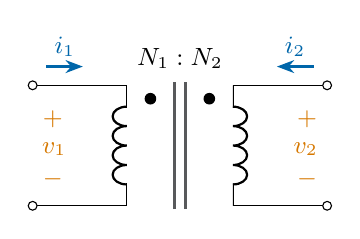
\begin{tikzpicture}[scale=0.85]
        \exXf
      \end{tikzpicture}
    \end{column}
    \begin{column}{0.5\textwidth}
      $\Tm = \ ?$\\[12pt]
      \onslide<2->{%
      $\vone = \dfrac{N_1}{N_2}\,\vtwo$\\[8pt]
      $\ione = -\dfrac{N_2}{N_1}\,\itwo = \dfrac{N_2}{N_1}\,(-\itwo)$\\[12pt]
      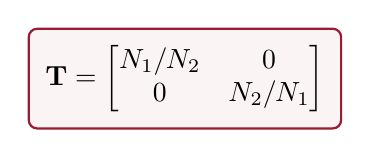
\begin{tikzpicture}
        \node[draw=metured, thick, fill=metured!5, rounded corners=3pt, inner sep=6pt]
          {$\Tm = \begin{bmatrix} N_1/N_2 & 0\\ 0 & N_2/N_1 \end{bmatrix}$};
      \end{tikzpicture}}
    \end{column}
  \end{columns}
\end{frame}

%--------------------------------------------------------------
\begin{frame}{Which test? Open or short}
  \vfill
  \begin{center}
  \small
  \renewcommand{\arraystretch}{1.45}
  \begin{tabular}{@{}l c c c@{}}
    \toprule
    \textbf{Matrix} & \textbf{Inputs} & \textbf{1st column} & \textbf{2nd column}\\
    \midrule
    $\Rm$ & $\ione$, $\itwo$ & port 2 \alert{open} & port 1 \alert{open}\\
    $\Gm$ & $\vone$, $\vtwo$ & port 2 \textbf{shorted} & port 1 \textbf{shorted}\\
    $\Hm$ & $\ione$, $\vtwo$ & port 2 \textbf{shorted} & port 1 \alert{open}\\
    $\Hm'$ & $\vone$, $\itwo$ & port 2 \alert{open} & port 1 \textbf{shorted}\\
    $\Tm$ & $\vtwo$, $-\itwo$ & port 2 \alert{open} & port 2 \textbf{shorted}\\
    \bottomrule
  \end{tabular}
  \end{center}
  \vfill
  \onslide<2->{%
  \begin{center}
    Zero the other input: \ $\Icol{i} = 0$ \ $\Rightarrow$ \ \alert{open}, \quad
    $\Vcol{v} = 0$ \ $\Rightarrow$ \ \textbf{short}
  \end{center}}
  \vfill
\end{frame}

%--------------------------------------------------------------
\begin{frame}{Measuring a two-port}
  \begin{columns}[t,onlytextwidth]
    \begin{column}{0.49\textwidth}
      \centering
      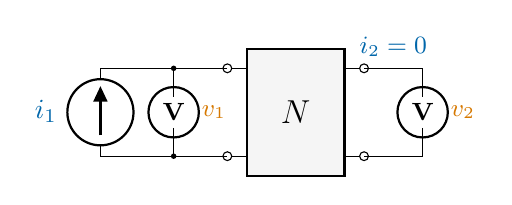
\begin{tikzpicture}[scale=0.62]
        \bench{0}
      \end{tikzpicture}\\[4pt]
      \textbf{Open-circuit test}\\[2pt]
      $r_{11} = \dfrac{\vone}{\ione}$, \quad $r_{21} = \dfrac{\vtwo}{\ione}$
    \end{column}
    \begin{column}{0.49\textwidth}
      \centering
      \onslide<2->{%
      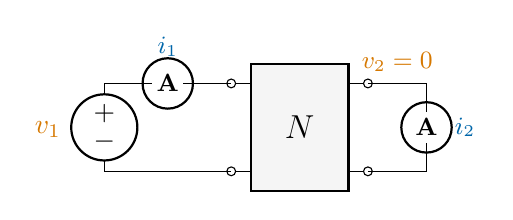
\begin{tikzpicture}[scale=0.62]
        \bench{1}
      \end{tikzpicture}\\[4pt]
      \textbf{Short-circuit test}\\[2pt]
      $g_{11} = \dfrac{\ione}{\vone}$, \quad $g_{21} = \dfrac{\itwo}{\vone}$}
    \end{column}
  \end{columns}
  \vfill
  \begin{itemize}\itemsep6pt
    \item Ideal voltmeter: \ an \alert{open}; \ ideal ammeter: \ a \textbf{short}
    \item<3-> One meter reading divided by the source value
  \end{itemize}
  \vfill
\end{frame}

%--------------------------------------------------------------
\begin{frame}{Example 14.7: $\Rm$ from two measurements}
  \begin{columns}[c,onlytextwidth]
    \begin{column}{0.5\textwidth}
      \centering
      \renewcommand{\arraystretch}{1.3}
      \begin{tabular}{@{}lcccc@{}}
        \toprule
         & $\ione$ & $\itwo$ & $\vone$ & $\vtwo$\\
        \midrule
        Exp.\ 1 & $1$ & $1$ & $5$ & $5$\\
        Exp.\ 2 & $1$ & $-1$ & $3$ & $-1$\\
        \bottomrule
      \end{tabular}\\[8pt]
      {\small No port open: \ $\Rm = \ ?$}
    \end{column}
    \begin{column}{0.48\textwidth}
      \onslide<2->{%
      $\begin{bmatrix} 5 & 3\\ 5 & -1 \end{bmatrix} = \Rm \begin{bmatrix} 1 & 1\\ 1 & -1 \end{bmatrix}$\\[10pt]}
      \onslide<3->{%
      $\Rm = \mathbf{V}\,\mathbf{I}^{-1} = \begin{bmatrix} 4 & 1\\ 2 & 3 \end{bmatrix}$\\[10pt]
      {\small Any two independent experiments}}
    \end{column}
  \end{columns}
\end{frame}

%==============================================================
\roadmapframe{7}

%--------------------------------------------------------------
\begin{frame}{The power of a two-port}
  \begin{columns}[c,onlytextwidth]
    \begin{column}{0.46\textwidth}
      \centering
      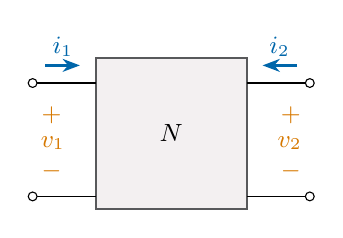
\begin{tikzpicture}[scale=0.8]
        \tpbox{$N$}
      \end{tikzpicture}
    \end{column}
    \begin{column}{0.52\textwidth}
      $P_N$: the sum of the powers of all elements inside $N$\\[12pt]
      \onslide<2->{%
      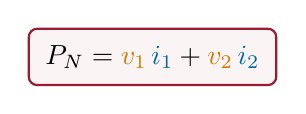
\begin{tikzpicture}
        \node[draw=metured, thick, fill=metured!5, rounded corners=3pt, inner sep=6pt]
          {$P_N = \vone\,\ione + \vtwo\,\itwo$};
      \end{tikzpicture}\\[8pt]
      {\small Proof: Tellegen's theorem (previously)}}
    \end{column}
  \end{columns}
  \vfill
  \onslide<3->{%
  \begin{itemize}\itemsep8pt
    \item \textbf{Passive:} $P_N \geq 0$ for all possible port variables
    \item \textbf{Active:} not passive
  \end{itemize}}
  \vfill
\end{frame}

%--------------------------------------------------------------
\begin{frame}{Example 14.8: is the ideal transformer passive?}
  \begin{columns}[c,onlytextwidth]
    \begin{column}{0.48\textwidth}
      \centering
      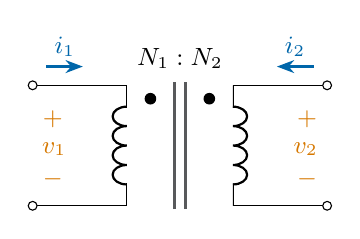
\begin{tikzpicture}[scale=0.85]
        \exXf
      \end{tikzpicture}
    \end{column}
    \begin{column}{0.5\textwidth}
      $P_N = \vone\,\ione + \vtwo\,\itwo$\\[8pt]
      \onslide<2->{%
      Plug $\vone = n\,\vtwo$, \ $\itwo = -n\,\ione$:\\[6pt]
      $P_N = n\,\vtwo\,\ione - n\,\vtwo\,\ione = 0$\\[12pt]
      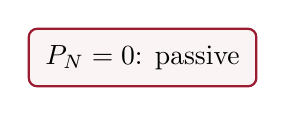
\begin{tikzpicture}
        \node[draw=metured, thick, fill=metured!5, rounded corners=3pt, inner sep=6pt]
          {$P_N = 0$: passive};
      \end{tikzpicture}\\[8pt]
      It neither absorbs nor delivers power}
    \end{column}
  \end{columns}
\end{frame}

%--------------------------------------------------------------
\begin{frame}{Summary}
  \vfill
  \begin{center}
  \renewcommand{\arraystretch}{1.6}
  \begin{tabular}{@{}>{\raggedright}p{3.0cm} >{\raggedright}p{4.6cm} >{\raggedright\arraybackslash}p{4.4cm}@{}}
    \toprule
    \textbf{Matrix} & \textbf{Equation} & \textbf{Tests}\\
    \midrule
    resistance $\Rm$ & $[\vone \ \vtwo]^T = \Rm\,[\ione \ \itwo]^T$ & ports open\\
    conductance $\Gm$ & $[\ione \ \itwo]^T = \Gm\,[\vone \ \vtwo]^T$ & ports shorted; $\Gm = \Rm^{-1}$\\
    hybrid $\Hm$ & $[\vone \ \itwo]^T = \Hm\,[\ione \ \vtwo]^T$ & port 2 shorted, port 1 open\\
    transmission $\Tm$ & $[\vone \ \ione]^T = \Tm\,[\vtwo \ {-\itwo}]^T$ & port 1 from port 2\\
    \bottomrule
  \end{tabular}
  \end{center}
  \vfill
  \begin{center}
    $P_N = \vone\,\ione + \vtwo\,\itwo$; \ passive if $P_N \geq 0$ always
  \end{center}
  \vfill
\end{frame}


\end{document}
